\section{Benchmarks}

\hidenum
\begin{frame}[noframenumbering]
\frametitle{Contents}
 \tableofcontents[currentsection,hideallsubsections]
\end{frame}
\shownum



\subsection{Benchmarks}

\begin{frame}
  \begin{block}{Non-Optimal Choices Throughout}
    \begin{enumerate}[<+-|alert@+>]
      \item Only libre software used (no MKL, ACML, etc.).
      \item 1 core = 1 MPI process.
      \item No tuning for data distribution.
    \end{enumerate}
  \end{block}
\end{frame}

\begin{frame}
  \begin{block}{Benchmark Data}
    \begin{enumerate}[<+-|alert@+>]
      \item Random normal $N(100, 10000)$.
      \item Local problem size of $\approx 43.4 MiB$.
      \item Three sets:  500, 1000, and 2000 columns.
      \item Several runs at different core sizes within each set.
    \end{enumerate}
  \end{block}
\end{frame}



% \subsection{Covariance}

\begin{frame}[fragile]
  \begin{block}{Covariance Code}
\begin{lstlisting}
x <- ddmatrix("rnorm", nrow=n, ncol=p, mean=mean, sd=sd)

cov.x <- cov(x)
\end{lstlisting}
  \end{block}
\end{frame}

\begin{frame}
  \begin{block}{\code{cov()}}
  \begin{center}
    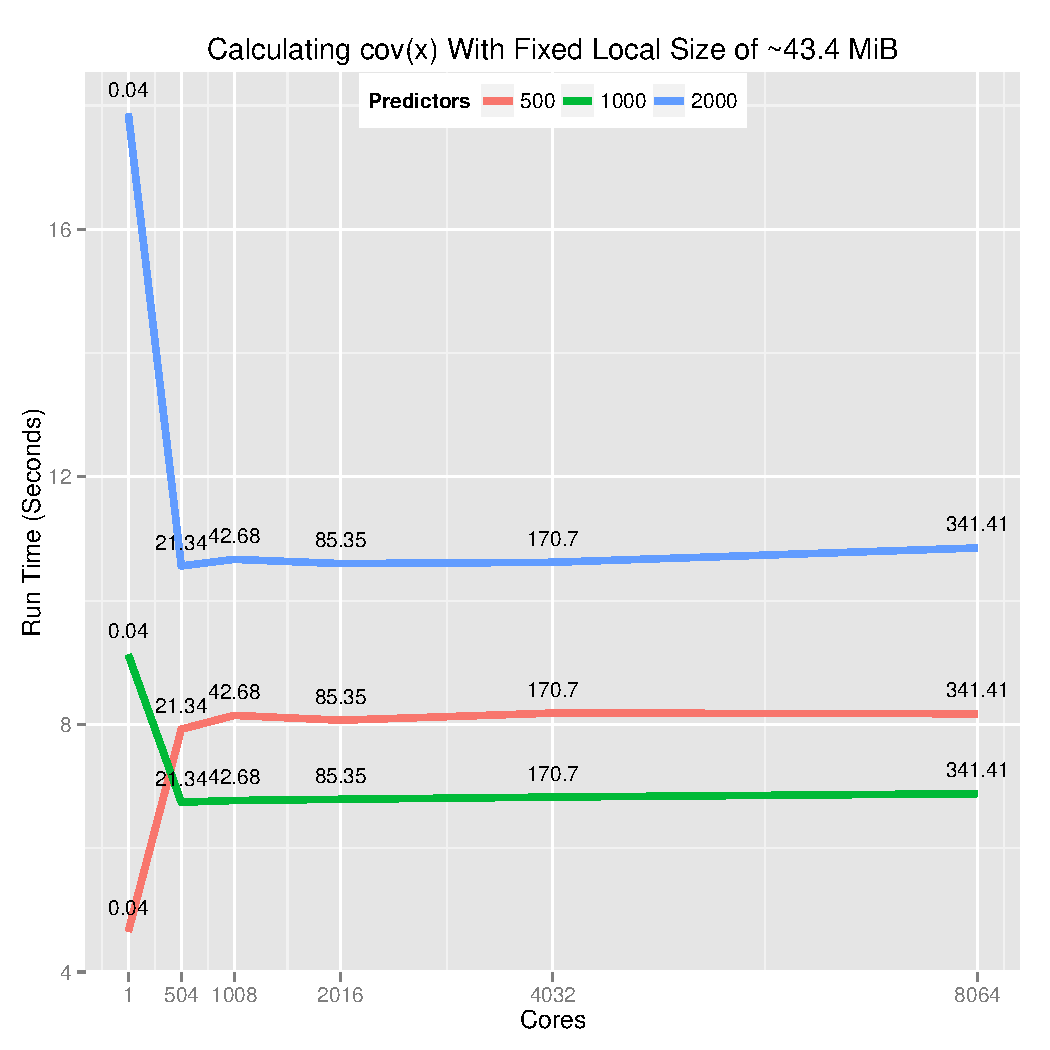
\includegraphics[height=.88\textheight]{pics/cov}
  \end{center}
  \end{block}
\end{frame}



% \subsection{Linear Model Fitting}

\begin{frame}[fragile]
  \begin{block}{Linear Model Code}
\begin{lstlisting}
x <- ddmatrix("rnorm", nrow=n, ncol=p, mean=mean, sd=sd)
beta_true <- ddmatrix("runif", nrow=p, ncol=1)

y <- x %*% beta_true

beta_est <- lm.fit(x=x, y=y)$coefficients
\end{lstlisting}
  \end{block}
\end{frame}

\begin{frame}
  \begin{block}{\code{Data Generation}}
  \begin{center}
    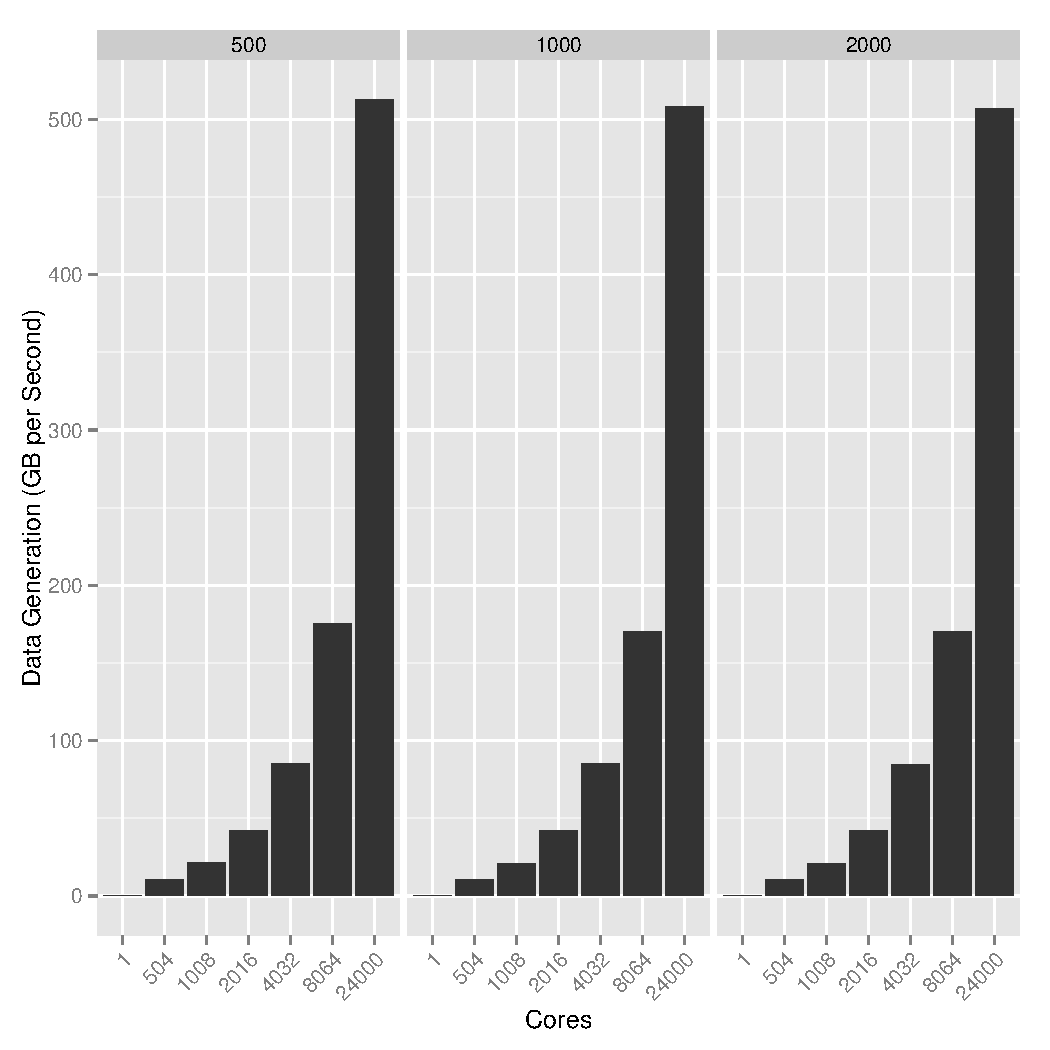
\includegraphics[height=.88\textheight]{pics/datagen}
  \end{center}
  \end{block}
\end{frame}

\begin{frame}
  \begin{block}{\code{lm.fit()}}
  \begin{center}
    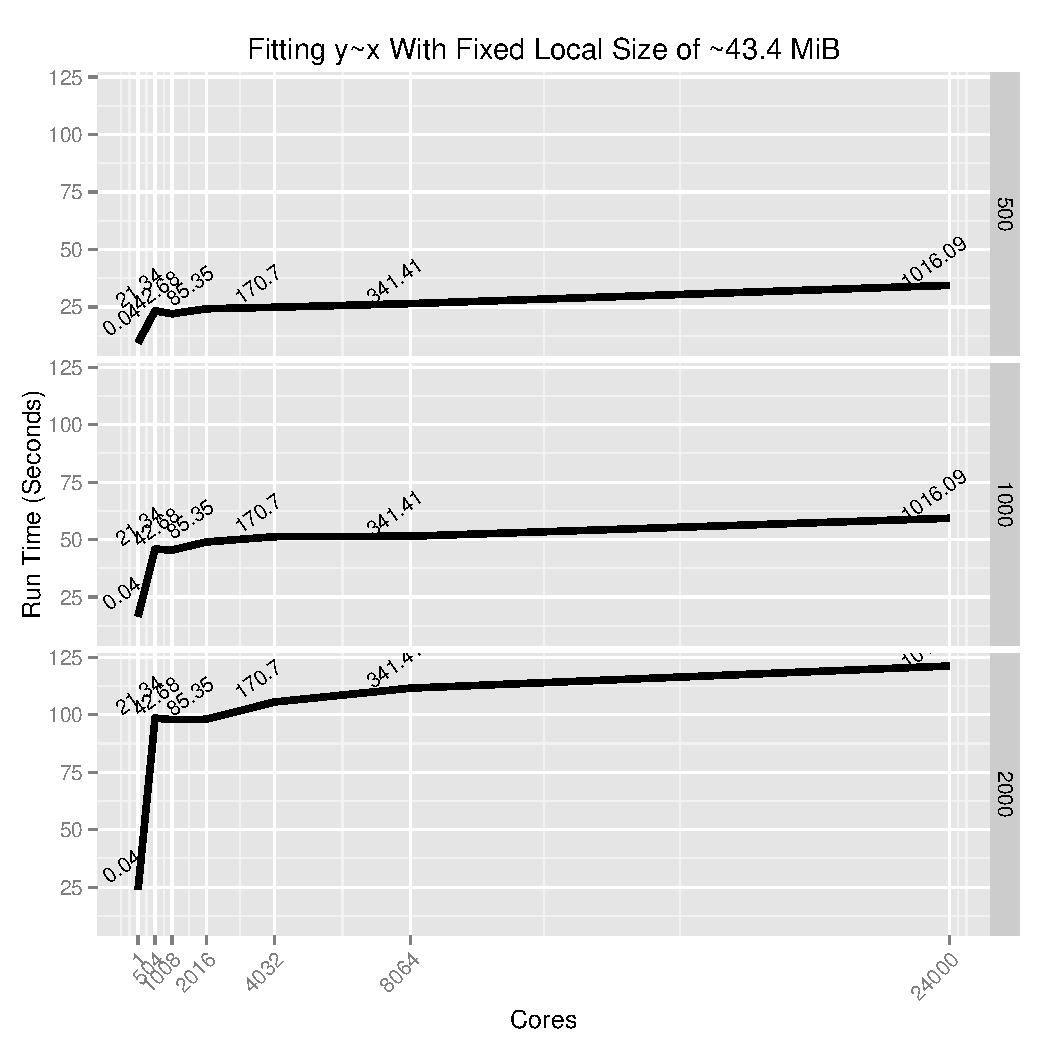
\includegraphics[height=.88\textheight]{pics/lmfit1}
  \end{center}
  \end{block}
\end{frame}

\begin{frame}
  \begin{block}{\code{lm.fit()}}
  \begin{center}
    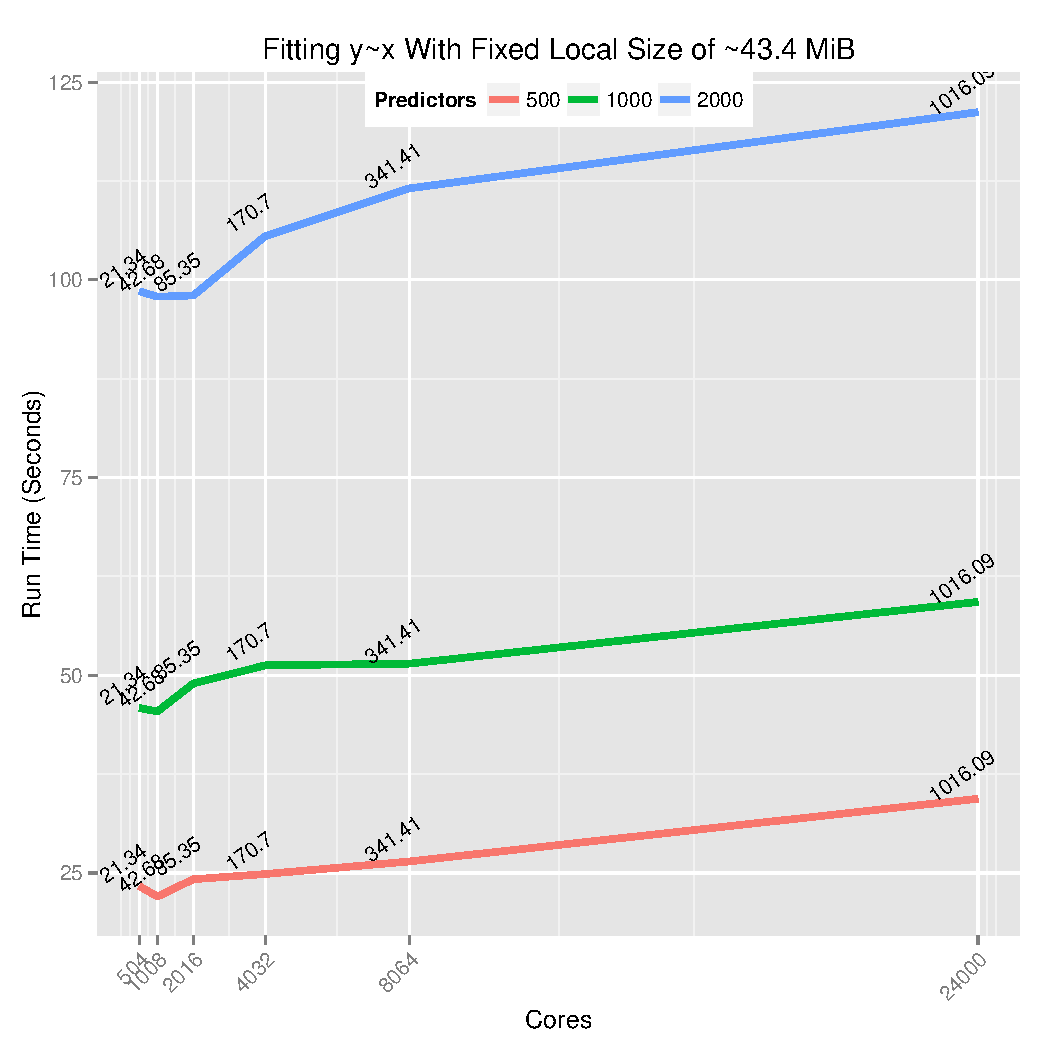
\includegraphics[height=.88\textheight]{pics/lmfit2}
  \end{center}
  \end{block}
\end{frame}